%%
%% Arquivo principal para:
%% - teses de doutorado
%% - dissertações de mestrado
%% - exames de qualificao de mestrado e doutorado
%%
%% NOTA: A PUBLICAÇÃO DESTE MODELO VISA APENAS ORIENTAR OS PÓS-GRADUANDOS
%% NA PREPARAÇÃO DE SEUS TEXTOS. O PPgEE DA UFRN NÃO PROVÊ ASSISTÊNCIA NO
%% USO DAS FERRAMENTAS NECESSÁRIAS AO USO DESTE MODELO (LATEX, XFIG, ETC.)
%%
%% Adelardo Medeiros, dezembro de 2005.

% DEFINIÇÕES GLOBAIS

% Esta primeira linha dá informações gerais sobre o documento.
% PARA A VERSÃO FINAL:
% papel A4, letra grande (12pt), openright (capítulos só iniciam em
% página direita, se necessário incluindo uma pgina em branco),
% twoside (o documento vai ser impresso em frente e costa)
\documentclass[a4paper,12pt,openright,twoside]{book}
% PARA A QUALIFICAÇÃO E PARA A VERSÃO INICIAL:
% papel A4, letra grande (12pt), openany (capítulos iniciam em
% qualquer página), oneside (o documento vai ser impresso só na frente)
%\documentclass[a4paper,12pt,openany,oneside]{book}

% PACOTES OBRIGATÓRIOS

% Use estes pacotes para poder digitar diretamente as letras com acento
% e para que a hifenização funcione corretamente
\usepackage[utf8]{inputenc}
\usepackage{ae}
% Para usar fontes standard ao invés das do LaTeX (gera melhores PDFs)
\usepackage{pslatex}
% Para a hifenização em português
\usepackage[portuges, brazil]{babel}
% Para que os primeiros parágrafos das seções também sejam indentados
\usepackage{indentfirst}
% Para poder incluir gráficos (figuras)
\usepackage{graphicx}
% Para poder fazer glossário ou lista de símbolos
% Use a segunda opção se quiser incluir na definição do símbolo a
% página e/ou a equação onde ela foi definida
% \usepackage[portuguese,noprefix]{nomencl}
%\usepackage[portuguese,noprefix,refeq,refpage]{nomencl}
% Para permitir espaçamento simples, 1 1/2 e duplo
\usepackage{setspace}
% Para usar alguns comandos matemáticos avançados muito úteis
\usepackage{amsmath}
% Para poder usar o ambiente "comment"
\usepackage{verbatim}
% Para poder ter tabelas com colunas de largura auto-ajustável
\usepackage{tabularx}
% Para executar um comando depois do fim da página corrente
\usepackage{afterpage}
% Para formatar URLs (endereços da Web)
\usepackage{url}
% Para reduzir os espaços entre os ítens (itemize, enumerate, etc.)
% Este pacote não faz parte da distribuição padrão do LaTeX.
\usepackage{noitemsep}
% Para as citações bibliográficas
\usepackage[abbr]{harvard}	% As chamadas são sempre abreviadas
\harvardparenthesis{square}	% Colchetes nas chamadas
\harvardyearparenthesis{round}	% Parêntesis nos anos das referências
%\renewcommand{\harvardand}{e}	% Substituir "&" por "e" nas referências

% PACOTES OPCIONAIS

% Para poder incluir arquivos Postscript com cores (do Xfig, por exemplo)
\usepackage{color}
% Para ter células em tabelas que ocupam mais de uma linha
\usepackage{multirow}
% Para poder ter tabelas longas em mais de uma página
%\usepackage{longtable}
% Para poder escrever partes do texto em "n" colunas
%\usepackage{multicol}
% Se você quiser personalizar os cabeçalhos das páginas
%\usepackage{fancyheadings}
% Para incluir algoritmos e listagens de códigos
%\usepackage{listings}
% Capítulos com títulos em um formato "decorado"
\usepackage{capitulos}

% As definiçõoes dos novos comandos estão agrupadas no arquivo "comandos.tex"
% Esta separação é opcional: se você preferir, pode por as definicoes
% diretamente neste arquivo
% newcommand define novos comandos, que podem passar a ser usados da
% mesma forma que os comandos LaTeX de base.

% Implica��o em f�rmulas
\newcommand{\implica}{\quad\Rightarrow\quad} %Meio de linha
\newcommand{\implicafim}{\quad\Rightarrow}   %Fim de linha
\newcommand{\tende}{\rightarrow}
\newcommand{\BibTeX}{\textsc{B\hspace{-0.1em}i\hspace{-0.1em}b\hspace{-0.3em}}\TeX}

% Fra��o com parentesis
\newcommand{\pfrac}[2]{\left(\frac{#1}{#2}\right)}

% Transformada de Laplace e transformada Z
%\newcommand{\lapl}{\makebox[0cm][l]{\hspace{0.1em}\raisebox{0.25ex}{-}}\mathcal{L}}
\newcommand{\lapl}{\pounds}
\newcommand{\transfz}{\mathcal{Z}}

% N�o aparecer o n�mero na primeira p�gina dos cap�tulos
\newcommand{\mychapter}[1]{\chapter{#1}\thispagestyle{empty}}

% Os cap�tulos sem n�mero
\newcommand{\mychapterast}[1]{\chapter*{#1}\thispagestyle{empty}
\chaptermark{#1}
\afterpage{\markboth{\uppercase{#1}}{\rightmark}}
\markboth{\uppercase{#1}}{}
}

% Se��es sem n�mero
\newcommand{\mysectionast}[1]{\section*{#1}
\addcontentsline{toc}{section}{#1}
\markright{\uppercase{#1}}
}

% No tabularx, as celulas devem ser centradas verticalmente
\renewcommand{\tabularxcolumn}[1]{m{#1}}

% C�lulas centralizadas horizontalmente no tabularx
\newcolumntype{C}{>{\centering\arraybackslash}X}

%% Abrevia figuras e tabelas
%\def\figurename{Fig.}
%\def\tablename{Tab.}


%
% As margens
%

% Direcao horizontal

% Margem interna
% Nas paginas impares
\setlength{\oddsidemargin}{3.5cm}         % Margem real desejada
% Nas paginas pares
\setlength{\evensidemargin}{2.5cm}        % Margem real desejada
% Largura do texto
\setlength{\textwidth}{15cm}
% As margens laterais no LaTeX sao sempre 1 polegada maiores do que as
% fixadas. Se foi fixada \setlength{\oddsidemargin}{3.5cm}, a margem
% real seria de 3.5+2.54=6.04cm. Para permitir que voce nao tenha que
% fazer esta conta, pode usar o numero desejado nas linhas anteriores
% e a gente subtrai 1in nas proximas linhas
\addtolength{\oddsidemargin}{-1in}
\addtolength{\evensidemargin}{-1in}
% Note que a margem direita nao e fixada diretamente:
% ela e obtida subtraindo-se os outros valores da largura da pagina.
% 3.5+15+x=21cm (largura A4) -> x = margem externa = 2.5cm

% Direcao vertical

% Margem superior (entre o topo da folha e o cabecalho), altura do
% cabecalho e distancia entre o fim do cabecalho e o inicio do texto
\setlength{\topmargin}{2.0cm}             % Margem real desejada
\setlength{\headheight}{1.0cm}
\setlength{\headsep}{1.0cm}
% Altura do texto (sem cabecalho e rodape)
\setlength{\textheight}{22.7cm}
% Distancia do fim do texto ao rodape
\setlength{\footskip}{1.0cm}
% A margem superior no LaTeX e sempre 1 polegada maior do que a
% fixada. Se foi fixada \setlength{\topmargin}{2.0cm}, a margem
%real seria de 2.0+2.54=4.54cm. Para permitir que voce nao tenha que
% fazer esta conta, pode usar o numero desejado na linha anterior
% e a gente subtrai 1in na proxima linha
\addtolength{\topmargin}{-1in}
% Note que a margem inferior nao e fixada diretamente:
% ela e obtida subtraindo-se os outros valores, sem incluir o
% "footskip", da altura da pagina.
% 2.0+1.0+1.0+22.7+x=29.7cm (altura A4) -> x = margem inferior = 3cm

%
% O estilo das referencias bibliograficas
%

\bibliographystyle{ppgee}

%
% O espacamento entre linhas
%

% As paginas iniciais sao sempre em espacamento simples
\singlespacing

% Para a criacao do glossario (ou lista de simbolos)
\makeglossary

% Lista de arquivos a serem processados. Estes comandos "includeonly" sao
% dispensaveis e devem obrigatoriamente ser comentados na hora de gerar o
% documento definitivo. Eles servem para compilar apenas parte do documento.
% e util, durante a redacao, para que nao se tenha de compilar todo o
% documento a cada vez que se faz uma alteracao. Por exemplo, se eu estou
% fazendo alteracoes na dedicatoria e as outras partes nao tem interesse no
% momento, posso incluir (descomentar) a linha "\includeonly{preambulo}"
%\includeonly{rosto}
%\includeonly{catalograficos}
%\includeonly{preambulo}
%\includeonly{resumos}
%\includeonly{introducao/introducao}
%\includeonly{estilo/estilo}
%\includeonly{matematica/matematica}
%\includeonly{figuras/figuras}
%\includeonly{conclusao/conclusao}
%\includeonly{apendice/apendice}

% Inicia o texto
\begin{document}

% Paginas iniciais (sem numeracao)
\pagestyle{empty}

% Pgina de rosto (capa interna)
%
% ********** Página de Rosto
%

% titlepage gera páginas sem numeração
\begin{titlepage}

\begin{center}

\small

% O comando @{} no ambiente tabular x é para criar um novo delimitador
% entre colunas que não a barra vertical | que é normalmente utilizada.
% O delimitador desejado vai entre as chaves. No exemplo, não há nada,
% de modo que o delimitador é vazio. Este recurso está sendo usado para
% eliminar o espaço que geralmente existe entre as colunas
% \begin{tabularx}{\linewidth}{@{}l@{}C@{}r@{}}
% A figura foi colocada dentro de um parbox para que fique verticalmente
% centralizada em relação ao resto da linha
% \parbox[c]{3cm}{\includegraphics[width=\linewidth]{FARN}} &
\begin{center}
\textsf{\textsc{Faculdade Natalense para o Desenvolvimento do Rio Grande do Norte}}
\end{center} % &
%% \parbox[c]{2cm}{\includegraphics[width=\linewidth]{figuras/dca}}
% \end{tabularx}

% O vfill é um espação vertical que assume a máxima dimensão possível
% Os vfill's desta página foram utilizados para que o texto ocupe
% toda a folha
\vfill

\LARGE

\textbf{Atualização de \textit{Web Services} em Tempo Real}

\vfill

\Large

\textbf{Vinícius Brandão Mendes}

\vfill

\normalsize

Orientador: Prof. Ricardo Wendel
% Se não houver co-orientador, comente a próxima linha
% \\[2ex] Co-orientador: Prof. Dr. Beltrano Catandura do Amaral

\vfill

\hfill
\parbox{0.5\linewidth}{\textbf{%
% Descomente as opçõs que se aplicam ao seu caso
%Proposta de Tema para Qualificação}
Relatório técnico}
%Tese de Doutorado}
apresentado ao Curso Especialização em Desenvolvimento
de Sistemas Corporativos da FARN
como trabalho de conclusão de curso.}
%Doutor em Ciências.}

\vfill

\large

% Este número de ordem deve ser obtido na coordenação do PPgEE
% Corresponde ao número sequencial da sua tese ou dissertação:
% por exemplo, a 25 tese de doutorado terá o número de ordem D25
% Evidentemente, este dado não existe para propostas de tema, caso
% em que a próxima linha deve ser comentada.
%Número de ordem PPgEE: M000

Natal, RN, abril de 2011

\end{center}

\end{titlepage}


% Ficha catalografica: os dados catalograficos devem ser fornecidos
% pela BCZM.
% So sao incluidos na versao final da tese ou dissertacao. Nao sao
% incluidos nem na proposta de tema de qualificacao nem na versao
% preliminar da tese ou dissertacao: nestes casos, comente a proxima linha.
%\include{catalograficos}

% Assinaturas da banca, dedicatoria e agradecimentos
% So sao incluidos na versao final da tese ou dissertacao. Nao sao
% incluidos nem na proposta de tema de qualificacao nem na versao
% preliminar da tese ou dissertacao: nestes casos, comente a proxima linha.
%% %
% ********** P�gina de assinaturas
%

\begin{titlepage}

\begin{center}

\LARGE

\textbf{Atualiza��o de cota��es atrav�s da consulta de \textit{Web Services} em tempo real}

\vfill

\Large

\textbf{Vin�cius Brand�o Mendes}

\end{center}

\vfill

% O \noindent � para eliminar a tabula��o inicial que normalmente �
% colocada na primeira frase dos par�grafos
\noindent
% Descomente a op��o que se aplica ao seu caso
% Note que propostas de tema de qualifica��o nunca t�m pre�mbulo.
Relat�rio t�cnico
%Tese de Doutorado
aprovado em \rule{.8cm}{.1mm} / \rule{.8cm}{.1mm} / \rule{1.6cm}{.1mm} pela banca examinadora composta
pelos seguintes membros:

% Os nomes dos membros da banca examinadora devem ser listados
% na seguinte ordem: orientador, co-orientador (caso haja),
% examinadores externos, examinadores internos. Dentro de uma mesma
% categoria, por ordem alfab?tica

\begin{center}

\vspace{1.5cm}\rule{0.95\linewidth}{1pt}
\parbox{0.9\linewidth}{%
Prof. Ricardo Wendell (Orientador) \dotfill\ FARN}

\vspace{1.5cm}\rule{0.95\linewidth}{1pt}
\parbox{0.9\linewidth}{%
Prof.  \dotfill\ FARN}

\vspace{1.5cm}\rule{0.95\linewidth}{1pt}
\parbox{0.9\linewidth}{%
Prof. \dotfill\ FARN}

\end{center}

\end{titlepage}

%
% ********** Dedicat�ria
%

% A dedicat�ria n�o � obrigat�ria. Se voc� tem algu�m ou algo que teve
% uma import�ncia fundamental ao longo do seu curso, pode dedicar a ele(a)
% este trabalho. Geralmente n�o se faz dedicat�ria a v�rias pessoas: para
% isso existe a se��o de agradecimentos.
% Se n�o quiser dedicat�ria, basta excluir o texto entre
% \begin{titlepage} e \end{titlepage}

% \begin{titlepage}

%\vspace*{\fill}

%\hfill
%\begin{minipage}{0.5\linewidth}
%\begin{flushright}
%\large\it
%Aos meus pais pela minha educa��o, orienta��o, apoio e aten��o dispensados a mim.
%\end{flushright}
%\end{minipage}
%
%\vspace*{\fill}

%\end{titlepage}

%
% ********** Agradecimentos
%

% Os agradecimentos n�o s�o obrigat�rios. Se existem pessoas que lhe
% ajudaram ao longo do seu curso, pode incluir um agradecimento.
% Se n�o quiser agradecimentos, basta excluir o texto ap�s \chapter*{...}

\chapter*{Agradecimentos}
\thispagestyle{empty}

\begin{trivlist}  \itemsep 2ex

\item Ao meu orientador, professor Ricardo Wendell, sou grato pela orienta��o.

\item Aos meus pais, Joalmi Mendes de Oliveira e Maria Gleide Brand�o Mendes, pelo apoio total durante a execu��o do trabalho e durante toda a minha vida, com educa��o, instru��o e companheirismo.

\item � minha noiva Rosana Curvelo de Souza pelo constante incentivo.

\item Ao colega F�bio Miranda Costa pelo apoio durante o curso.

\item Aos meus irm�os, familiares e amigos pela paci�ncia e apoio dispensados durante a execu��o do trabalho.

\end{trivlist}


%
% O espaamento entre linhas
%

% PARA A VERSO FINAL:
% Deve ser usado espaamento simples nas pginas de texto
\singlespacing
% PARA A QUALIFICAO E PARA A VERSO INICIAL:
% Deve ser usado espaamento 1 1/2 nas pginas de texto
%\onehalfspacing

% Resumo/Abstract
%% %
% ********** Resumo
%

% Usa-se \chapter*, e n�o \chapter, porque este "cap�tulo" n�o deve
% ser numerado.
% Na maioria das vezes, ao inv�s dos comandos LaTeX \chapter e \chapter*,
% deve-se usar as nossas vers�es definidas no arquivo comandos.tex,
% \mychapter e \mychapterast. Isto porque os comandos LaTeX t�m um erro
% que faz com que eles sempre coloquem o n�mero da p�gina no rodap� na
% primeira p�gina do cap�tulo, mesmo que o estilo que estejamos usando
% para numera��o seja outro.
\mychapterast{Resumo}

Neste trabalho ser� relatada a integra��o entre um portal de internet e uma fonte de cota��es que disponibiliza dados atrav�s de um \textit{web service} baseado em SOAP (\textit{Simple Object Access Protocol}) de forma a ter o menor tempo de resposta ao usu�rio com o dado o mais atualizado poss�vel. Foram abordadas tr�s t�cnicas: requisi��es ao \textit{web service} sob demanda do usu�rio; atualizador com requisi��es s�ncronas e sequenciais em um �nico processo; e atualizador com requisi��es s�ncronas em v�rios processos.

\vspace{1.5ex}

{\bf Palavras-chave}: \textit{Web services}, SOAP, computa��o distribu�da, programa��o concorrente.
%
% ********** Abstract
%

\mychapterast{Abstract}

On the following work, will be reported the integration between an internet portal and a data source that makes the data available through a web service based on SOAP in a way that it can keep the minimum response time to the user with the most recent data. Three techniques were considered: request to the web service on user demand; updater with synchronous and sequential requests in a single process; and updater with synchronous requests with multiprocessing.

\vspace{1.5ex}

{\bf Keywords}: Web Services, SOAP, distributed computing, multiprocessing.


% Paginas introdutrias (com numerao romana)
\frontmatter

% Lista de contedo (sumrio, gerado automaticamente)
\addcontentsline{toc}{chapter}{Sumário}
\tableofcontents

% Lista de figuras (gerada automaticamente)
\cleardoublepage
\addcontentsline{toc}{chapter}{Lista de Figuras}
\listoffigures

% Lista de tabelas (gerada automaticamente)
%\cleardoublepage
%\addcontentsline{toc}{chapter}{Lista de Tabelas}
%\listoftables

% Glossrio (gerado automaticamente - veja entradas em
% introducao/introducao.tex e em estilo/estilo.tex)
%\cleardoublepage
%\renewcommand{\nomname}{Lista de Smbolos e Abreviaturas}
%\markboth{\MakeUppercase{\nomname}}{\MakeUppercase{\nomname}}
%\addcontentsline{toc}{chapter}{\nomname}
% O argumento opcional do comando \printglossary  a largura deixada
% para os smbolos no glossrio. Se seus smbolos so "largos", como
% neste exemplo,   melhor por mais espao do que o 1cm que  reservado
% por default
% \printglossary[1.5cm]

% Pginas do texto principal (com cabealho)
\mainmatter
\pagestyle{headings}

% Para facilitar a organizao, foi criado um diretrio para cada
% captulo do documento, pois assim os arquivos das figuras ficam
% classificados por captulos

%% %%
%% Captulo 1: Modelo de Captulo
%%

% Est sendo usando o comando \mychapter, que foi definido no arquivo
% comandos.tex. Este comando \mychapter  essencialmente o mesmo que o
% comando \chapter, com a diferena que acrescenta um \thispagestyle{empty}
% aps o \chapter. Isto é necessário para corrigir um erro de LaTeX, que
% coloca um número de pgina no rodapé de todas as páginas iniciais dos
% capítulos, mesmo quando o estilo de numeração escolhido é outro.
\mychapter{Introdução}
\label{Cap:introducao}

Este trabalho trata de um cliente de \textit{Web Service} SOAP que deve obter o mais rapidamente possível uma grande quantidade de dados do servidor e persistí-los em seu banco de dados. Existem inúmeras formas de resolver esse problema. Neste trabalho serão abordadas algumas técnicas possíveis.

\section{Descrição geral}

O trabalho é baseado em um \textit{Web Service} SOAP, que é um protocolo para troca de informações estruturadas em uma plataforma descentralizada e distribuída.

Um portal de internet precisa oferecer a seus usuários em tempo real dados que são obtidos através de um servidor que os fornece através de um \textit{web service}. Para não ter atraso na informação oferecida, ele precisa requisitar ao fornecedor de dados o mais frequentemente possível ao mesmo tempo que tem que manter um bom tempo de resposta para seus usuários.

\section{Objetivo}

O objetivo do trabalho é resolver os problemas relacionados à otimização do tempo de resposta e à frequência de atualização do dado. Por se tratar de um problema de otimização de tempo de resposta é necessário pensar na latência e no \textit{overhead} gerado por uma conexão HTTP e analisar a melhor arquitetura de sistema possível.

\section{Motivação}

Com o avanço da informática e de conceitos como a computação em nuvem, cada vez mais os servidores estão em constante comunicação ao redor do mundo. Seja para autenticar usuários, seja para persistir dados ou seja para solicitar dados. Um portal de notícias, por exemplo, exibe, além das notícias, dados meteorológicos e econômicos. Esses dados normalmente não são produzidos pelo próprio portal e então são necessárias parcerias com fornecedores de conteúdo que disponham de tal informação. Estes fornecedores, em geral, disponibilizam os dados através de um \textit{Web Service}.

Dado que no mundo jornalístico a agilidade na entrega de informações é um fator primordial para o sucesso, surge a necessidade de otimizar o tempo de consumo de tais fornecedores a fim de entregar aos usuários a informação mais recente possível.

\section{Metodologia}

O projeto foi dividido em três partes: 

\begin{itemize}
\item módulo para realizar comunicação utilizando SOAP;
\item estratégia de atualização de dados sob demanda;
\item atualizador de dados independente de este ser requisitado ou não.
\end{itemize}


\subsection{Módulo para realizar comunicação utilizando SOAP}

Foi necessário desenvolver um módulo capaz de fazer a comunicação utilizando o protocolo SOAP, serví-los aos clientes e persistí-los em seu banco de dados.

\subsection{Estratégia de atualização de dados sob demanda}

Uma das possíveis opções de atualização de dados é fazê-lo sob demanda. A medida em que um usuário solicita o dado, o portal o requisita ao fornecedor e gera a resposta para o usuário. Esta foi a primeira estratégia analisada.

\subsection{Atualizador de dados independente de este ser requisitado ou não}

A atualização de dados sob demanda leva a um tempo de resposta muito alto para o usuário. Então foi analisada uma nova estratégia de atualizar os dados indepentementemente de eles terem sido requisitados pelos usuários ou não. Esta estratégia se mostrou mais interessante por reduzir o tempo de resposta para o usuário.



%% \include{arquitetura/arquitetura}

%% \include{cores/cores}

%% \include{calibracao/calibracao}

%% \include{rotulo/rotulo}

%% \mychapter{Implementa��o}
\label{Cap:implementacao}

A implementa��o foi feita utilizando a linguagem de programa��o Python. Foi escolhido um cliente para o protocolo SOAP e encontrada uma API que disponibiliza cota��es de moedas atrav�s de um \textit{web service} que utiliza este protocolo.

\section{Por que Python?}

Python � uma linguagem interpretada, din�mica e fortemente tipada. Por ter estas caracter�sticas torna o trabalho mais r�pido e diminui o tempo de desenvolvimento do projeto, que no caso � apenas uma prova de conceito, portanto o tempo curto de desenvolvimento � bastante interessante. Isso n�o significa que Python seja uma linguagem apropriada apenas para provas de conceito, visto que grandes empresas adotam esta tecnologia em seus projetos que est�o hoje em produ��o.

\section{Cliente SOAP}

Para obten��o das cota��es do \textit{web service} foi utilizada a biblioteca Suds \cite{ref-suds} para fazer a interface entre o c�digo Python e a API externa. A biblioteca reconhece o WSDL e gera classes Python para acesso remoto ao \textit{web service}.

\subsection{API que disponibiliza cota��es}

A API disponibiliza um �nico m�todo para obten��o da cota��o de uma moeda em rela��o a uma outra. Para simplificar a implementa��o, as cota��es foram todas normalizadas para sempre serem em rela��o ao D�lar Americano.

\section{Estrat�gias de utiliza��o do cliente}

Foram desenvolvidas duas implementa��es para o problema com o objetivo de encontrar a mais perform�tica:

\begin{itemize}
\item atualiza��o de dados sob demanda;
\item atualizador de dados independente de demanda.
\end{itemize}

\subsection{Atualiza��o de dados sob demanda}

\begin{figure}[htbp!] \begin{center}
% fbox faz uma borda ao redor do seu argumento
\fbox{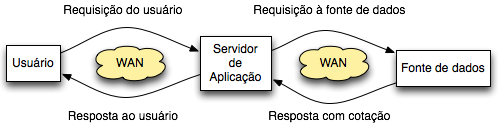
\includegraphics[width=0.95\linewidth]{img/requisicoes_sob_demanda}}
\caption{Arquitetura da solu��o com atualiza��o de dados sob demanda.}
\label{Fig:atualizacao_sob_demanda}
\end{center} \end{figure}

Um das implementa��es testadas foi conectar � API para obter uma cota��o apenas quando o usu�rio requisitasse. Isso evita a atualiza��o de cota��es que n�o est�o sendo requisitadas por usu�rio nenhum. Em contrapartida, o tempo de resposta ao usu�rio ser� alto, visto que ser� acrescido ao tempo de processamento, o tempo da requisi��o � fonte de dados, que � atrav�s da internet e, portanto, lenta.

Um outro problema neste caso � que a requisi��o � fonte de dados � bloqueante e ser� processada pelo mesmo processo utilizado para receber e responder a requisi��o do usu�rio, o que faz com que processos que deveriam responder usu�rios fiquem ocupados com requisi��es a fontes de dados externas, diminuindo o n�mero de usu�rios atendidos por segundo.

\subsection{Atualizador de dados independente de demanda}

\begin{figure}[htbp!] \begin{center}
% fbox faz uma borda ao redor do seu argumento
\fbox{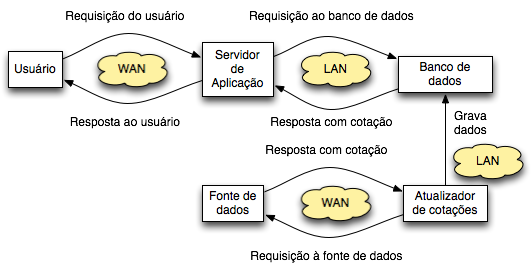
\includegraphics[width=0.95\linewidth]{img/atualizador}}
\caption{Arquitetura da solu��o com atualizador de dados independente de demanda.}
\label{Fig:atualizador}
\end{center} \end{figure}

A segunda implementa��o testada foi desenvolver um sistema cuja fun��o � requisitar as cota��es � fonte de dados em uma frequ�ncia determinada e salv�-las em um banco de dados. Desta forma, a cada requisi��o de usu�rio, o sistema iria fazer apenas consultas ao banco de dados, que s�o muito mais r�pidas que acessar uma fonte de dados externa. Este processo pode ser visto no diagrama de sequ�ncia da figura~\ref{Fig:diagrama_sequencia_banco_de_dados}.

\begin{figure}[htbp!] \begin{center}
% fbox faz uma borda ao redor do seu argumento
\fbox{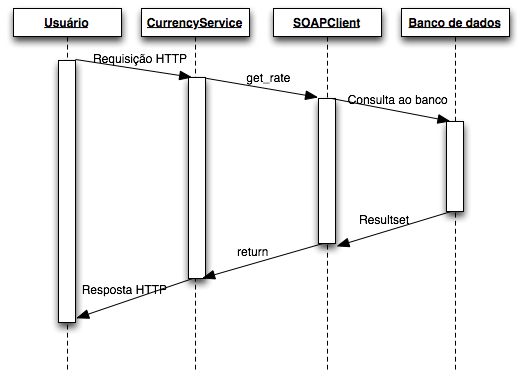
\includegraphics[width=0.95\linewidth]{img/diagrama_sequencia_banco_de_dados}}
\caption{Diagrama de sequ�ncia da requisi��o de um usu�rio ao sistema.}
\label{Fig:diagrama_sequencia_banco_de_dados}
\end{center} \end{figure}

Outra vantagem � que o banco de dados faz o papel de \textit{cachear} os dados e mesmo que exista falha na comunica��o com a fonte de dados, os usu�rios continuar�o recebendo os dados, mesmo que desatualizados. O fato dados serem salvos em um banco de dados tamb�m possibilita que a aplica��o que vai consumir esses dados seja em qualquer linguagem de programa��o, seja Java, Ruby, Python ou qualquer outra que possibilite a comunica��o com o banco de dados. No caso, o sistema que consome os dados do banco de dados foi desenvolvido em Python, utilizando a biblioteca CherryPy \cite{ref-cherrypy} como handler HTTP. O sistema foi feito utilizando o padr�o MVC \cite{ref-mvc}.

Como ponto fraco, o sistema deve atualizar todas as cota��es, mesmo as que n�o s�o demandadas t�o frequentemente pelos usu�rios. Isso pode gerar desperd�cio de poder computacional.

Esse sistema pode ou n�o utilizar m�ltiplos processos. Para o caso de um sistema multiprocessado, foi utilizada a biblioteca \textit{multiprocessing}, que � nativa da linguagem Python. No caso, o processo pai obt�m a lista de todas as cota��es a serem obtidas, e as passa para os processos filhos para que eles fa�am o trabalho de comunica��o com a fonte de dados.

A atualiza��o de uma cota��o � feita de acordo com o diagrama de sequ�ncia da figura~\ref{Fig:diagrama_sequencia_atualizador}. Cada processo repete este procedimento at� que o processo pai n�o tenha mais cota��es para serem atualizadas.

\begin{figure}[htbp!] \begin{center}
% fbox faz uma borda ao redor do seu argumento
\fbox{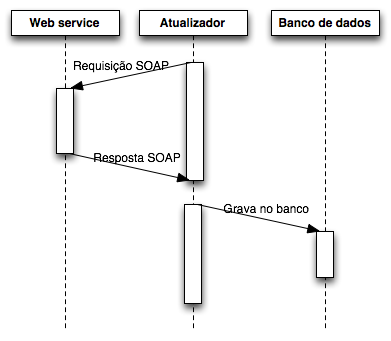
\includegraphics[width=0.95\linewidth]{img/diagrama_sequencia_atualizador}}
\caption{Diagrama de sequ�ncia da atualiza��o de uma cota��o.}
\label{Fig:diagrama_sequencia_atualizador}
\end{center} \end{figure}


%% \mychapter{Resultados}
\label{Cap:resultados}

\section{Requisi��es sob demanda}

\section{Atualizar todos os dados de tempos em tempos}

\subsection{Requisi��es sequenciais}

\subsection{Requisi��es paralelas com m�ltiplos processos}



%% \mychapter{Conclus�o}
\label{Cap:conclusao}



% Referncias bibliogficas (geradas automaticamente)
\addcontentsline{toc}{chapter}{Referncias bibliogrficas}
\bibliography{bibliografia}

%\appendix

%Apndice A 
% \include{apendice/apendice}

\end{document}
